%
% fig-bipolar.tex
%
% (c) 2025 Prof Dr Andreas Müller
%
\begin{figure}
\centering
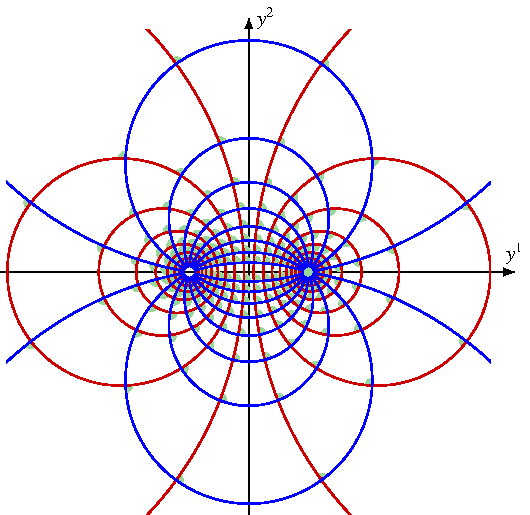
\includegraphics{papers/diffortho/images/bipolar.pdf}
\caption{Die Feldlinien und Äquipotentiallinien des Potentials
zweier Punktladungen in den Punkten $(\pm 1,0)$ können als Real-
und Imaginärteil der komplexen Funktion $y^1 + iy^2=\coth(x^1+ix^2)$ 
erzeugt werden.
Da komplexe Funktionen konforme Abbildungen der Ebene darstellen,
ist das $x^1$-$x^2$-Koordinatensystem orthogonal.
\label{diffortho:fig:bipolar}}
\end{figure}
